\documentclass[10pt]{hackr26}

% TikZ is not guaranteed by the class. float gives [H]. booktabs gives table rules.
\usepackage{tikz}
\usepackage{float}
\usepackage{booktabs}

%----------------------- Macros and Definitions --------------------------
% The environments theorem, lemma, cor, obs, conj, prop, defini and proof
% come from hackr26.cls.

%----------------------- Title -------------------------------------------

\title{The Minimum Tileset Problem for $2\times n$ Rectangles}

% TODO: authors
\author{
    firstname1 lastname1
    \thanks{Department of Computer Science, University of Texas Rio Grande Valley, {\tt name1@utrgv.edu}}
    \and
    firstname2 lastname2
    \thanks{Department of Computer Science, University of Texas Rio Grande Valley, {\tt name2@utrgv.edu}}
}

% Add the appropriate index information!

\index{lastname1, firstname1}
\index{lastname2, firstname2}

%------------------------------ Text -------------------------------------

\begin{document}
\maketitle
%%%%%%%%%%%%%%%%%%%%%%%%%%%%%%%%%%%%%%%%%%%%%%%%%%%%%%%%%%%%%%%%%%%%%%%%%%%%%%%%%%%%
\begin{abstract}
We study the number of tile types needed to uniquely self-assemble a $2\times n$ rectangle in the abstract Tile Assembly Model (aTAM).
At temperature 2, the answer is $\Theta(\sqrt n)$ for every seed position.
The lower bound is known, and the interior-seed upper bound is a sketch.
We add a comb with $n+1$ types for every seed cell and a two-row counter with about $3.46\sqrt n$ types, hand-traced but not machine-simulated.
For unary input, Mahaney's theorem shows that the problem is not NP-complete unless P $=$ NP.
We also give a $2^{O(\sqrt n\log n)}$ exact algorithm and an about 8-approximation.
The exact values for the interior seed and for temperature 1 stay open.
\end{abstract}
%%%%%%%%%%%%%%%%%%%%%%%%%%%%%%%%%%%%%%%%%%%%%%%%%%%%%%%%%%%%%%%%%%%%%%%%%%%%%%%%%%%
\section{Introduction and Model} \label{sec:intro}

The Minimum Tileset Problem asks for the fewest tile types that uniquely self-assemble a given shape.
The general problem is NP-complete, and it is polynomial for squares at temperature 2 and at every temperature.\footnote{The NP-completeness is due to Adleman et al.\ (STOC 2002), which we read only in abstract form. % TODO verify: S-MTS-1 partial (abstract only), not cited in the bibliography
}
% src: S-MTS-1, S-MTS-4
The square result is from~\cite{CDS11}.
% src: S-MTS-4
The strict (non-directed) variant is $\Sigma_2^P$-complete~\cite{BCDKS11}.
% src: S-MTS-3
We ask for the complexity of the directed problem on $2\times n$ rectangles.
Our answer is a tight $\Theta(\sqrt n)$ range on the number of types, plus two complexity statements.

\paragraph{Model.}
A tile type is a unit square with a glue label on each of its four sides (N, E, S, W), and a glue function gives each label a strength.
% src: S-MTS-4
Tiles never rotate and are placed by translation only.
At temperature $\tau$, a tile attaches when its matching sides have total strength at least $\tau$.
% src: S-MTS-2
One seed tile sits at a fixed cell, and growth starts there.
We call a system \emph{directed} if it has exactly one terminal assembly and that assembly has the target shape.
% src: S-MTS-4
Let $t$ be the least number of tile types of a directed system for $2\times n$ at a stated $\tau$ and seed cell.
We state $\tau$ for every result.
Where input size matters, $n$ is given in unary or as a sorted list of cells, and $s$ is in unary or fixed width.
The number $k$ may be in binary, since the reduction in Section~\ref{sec:cx} rewrites it.

%%%%%%%%%%%%%%%%%%%%%%%%%%%%%%%%%%%%%%%%%%%%%%%%%%%%%%%%%%%%%%%%%%%%%%%%%%%%%%%%%%%%
\section{Results} \label{sec:res}

Table~\ref{tab:results} lists every bound with its true status.
The two-row answer is $\Theta(\sqrt n)$ at $\tau=2$ for each seed position.

\begin{table}[H]
\centering
\small
\setlength{\tabcolsep}{3pt}
\begin{tabular}{@{}p{3.6cm}p{1.9cm}p{3.5cm}p{6.2cm}@{}}
\toprule
Setting & Lower & Upper & Status \\
\midrule
$2\times1$, any $\tau$ & 2 & 2 & proved (Thm.~\ref{thm:one}) \\
\midrule
$2\times n$, any $\tau$, any seed cell & $\sqrt n/2$ & $n+1$ (comb) & lower: \cite{ACG05}. Upper: proved (Thm.~\ref{thm:comb}) \\
\midrule
$\tau=2$, corner seed & $\sqrt n/2$ & $4\lceil\sqrt n\rceil+2$ & proved \cite{ACG05} \\
\midrule
$\tau=2$, corner seed, $n=1+mD$ & $\sqrt n/2$ & $m+3D+2\approx3.46\sqrt n$ & construction, hand-traced, not machine-simulated \\
\midrule
$\tau=2$, interior seed & $\sqrt n/2$ & $4\sqrt2\,\sqrt n+O(1)$ & upper bound is a sketch \\
\midrule
$\tau=1$, no mismatches & $n+1$ & $n+1$ & exact, from a source we read only in part \\
\midrule
$\tau=1$, general & $\Omega(\sqrt n)$ & $n+1$ & exact value open \\
\bottomrule
\end{tabular}
\caption{Bounds on the number of tile types $t$ for a directed $2\times n$ rectangle. Why: it separates what is proved from what is only sketched or hand-traced.}
\label{tab:results}
\end{table}
% src: S-MTS-2, S-MTS-5

\subsection{Small cases and the comb}

\begin{theorem}\label{thm:one}
For every $\tau\ge1$, the $2\times1$ rectangle needs exactly 2 tile types.
\end{theorem}
\begin{proof}
Take one type with glues N and S.
The second tile binds to the seed through one side, so that glue has strength at least $\tau$.
Then N and S carry the same label, and a third copy attaches above the second.
Growth never stops.
Two types suffice: $A$ has north glue $a$ of strength $\tau$, and $B$ has south glue $a$.
All other sides are null.
\end{proof}

\begin{theorem}\label{thm:comb}
For every $\tau\ge1$, every $n$ and every seed cell, a $2\times n$ rectangle is directed by $n+1$ tile types.
\end{theorem}
\begin{proof}
Let the bottom row use types $B_1,\dots,B_n$.
Type $B_i$ has east glue $e_i$ for $i<n$, west glue $e_{i-1}$ for $i>1$, and north glue $u$.
One top type $T$ has south glue $u$.
Every other side is null, and every glue has strength $\tau$.
Take the seed $B_s$.
East of it, only $B_{s+1}$ has west glue $e_s$.
West of it, only $B_{s-1}$ has east glue $e_{s-1}$.
By induction, each bottom cell has one candidate.
Each top cell offers only $T$, and the null east and west sides of $T$ stop growth.
So the terminal assembly is unique with shape $2\times n$.
A top-row seed breaks this set, because the $n$ bottom types compete under the seed $T$.
Use the vertically flipped comb: top types $T_1,\dots,T_n$ with the chain glues $e_i$ and south glue $u$, and one bottom type $B$ with north glue $u$.
The same induction applies.
\end{proof}

\begin{figure}[H]
\centering
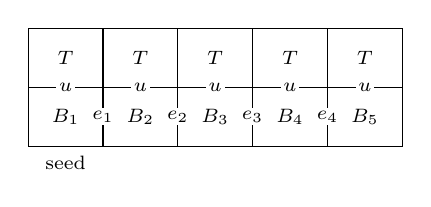
\begin{tikzpicture}[x=0.95cm,y=0.75cm,font=\scriptsize]
  \foreach \i in {1,...,5}{
    \draw (\i-1,0) rectangle (\i,1) node[midway]{$B_\i$};
    \draw (\i-1,1) rectangle (\i,2) node[midway]{$T$};
    \node[fill=white,inner sep=1pt] at (\i-0.5,1) {$u$};
  }
  \foreach \i in {1,...,4}{
    \node[fill=white,inner sep=1pt] at (\i,0.5) {$e_\i$};
  }
  \node[below] at (0.5,0) {seed};
\end{tikzpicture}
\caption{The comb for $n=5$ with the seed at $B_1$. Why: the five bottom tiles are chained by $e_i$, and all five share one top type $T$.}
\label{fig:comb}
\end{figure}

\subsection{Lower bound and corner upper bound}

\begin{theorem}[\cite{ACG05}, Thm.~3.1]\label{thm:lower}
At every $\tau$ and wherever the seed lies, a directed $2\times n$ system has $t\ge\sqrt n/2$.
\end{theorem}
% src: S-MTS-2
We do not re-prove it.
The proof finds three identically placed columns with the same attachment order, two on one side of the seed, and pumps the stretch between them.
% src: S-MTS-2
For a corner seed at $\tau=2$, a base-$m$ two-digit counter with $m=\lceil\sqrt n\rceil$ gives $t\le4\lceil\sqrt n\rceil+2$~\cite{ACG05}.
% src: S-MTS-2
For $n=100$, this reads $5\le t\le42$.
Thus the answer is $\Theta(\sqrt n)$ at $\tau=2$ for a corner seed, and the constants differ by a factor of about 8.

\subsection{A leaner two-row counter}

\paragraph{Construction (hand-traced, not machine-simulated).}
Let $n=1+mD$ with $m\ge2$ and $D\ge1$.
The seed $Z$ is the bottom tile of the east column, and growth runs west in $D$ blocks of $m$ columns.
The bottom row counts the position in a block with a chain $P_1,\dots,P_m$.
Here $P_j$ has west glue $p_j$ and $P_{j+1}$ has east glue $p_j$, both of strength 2.
Strength 2 is needed, since strength 1 would deadlock $P_{j+1}$ against the tile above it.
The top row holds a digit $d$ that counts blocks down from $D-1$ to $0$.
Each $d$ has its own strength-1 label $\delta_d$ and a strength-2 label $r_d$.
A shared digit label would let two digit tiles fit one cell.
The block cycle has five steps.
\begin{enumerate}
  \item Start tile $S_d$ attaches on $r_d$ alone.
  \item $P_1$ attaches under it on $q+s$ with strengths $1+1$.
  \item $P_2,\dots,P_m$ follow on the strength-2 chain glues.
  \item Middle tile $M_d$ fills each top cell on $\delta_d+g$.
  \item Decrement tile $X_d$ closes the block on $\delta_d+b$ and emits $r_{d-1}$.
\end{enumerate}
After $X_0$, no start tile exists, and $P_1$ sees only $q$ of strength 1, so growth stops.
The tile types are $m$ of type $P$, $D$ each of $S$, $M$, $X$, and two seed-column tiles $Z$ and $Y$, so $m+3D+2$ in all.
Setting $m=3D$ gives $2\sqrt{3n}\approx3.46\sqrt n$ types, against $4\sqrt n+2$ in~\cite{ACG05}.
We traced the construction by hand for $(m,D)=(3,2)$ and $(12,4)$.
For $(12,4)$, $n=49$ and the count is 26, against 50 for the comb.
For $D=58$ and $m=173$, $n=10{,}035$ and the count is 349.
The construction covers only $n=1+mD$, and other lengths need a partial first block that we did not work out.
We claim it as a construction, not as a theorem.

\subsection{Interior seed and temperature 1}

\begin{prop}[sketch]\label{prop:interior}
At $\tau=2$ and seed column $s$, $t\le4\lceil\sqrt a\rceil+4\lceil\sqrt b\rceil+O(1)\le4\sqrt2\,\sqrt n+O(1)$, where $a=s-1$ and $b=n-s$.
\end{prop}
\noindent\emph{Sketch.}
Grow one counter west and its mirror image east, sharing the seed column and using disjoint glue labels.
The step to the second inequality is $\sqrt a+\sqrt b\le\sqrt{2(a+b)}$.
The sketch relies on the claim of~\cite{ACG05} (p.~8) that the counter handles every arm length from 1 to $m^2$, which we did not re-check.
For a top-row seed cell, flip the construction vertically.
With Theorem~\ref{thm:lower}, this gives $\Theta(\sqrt n)$ at $\tau=2$ for every seed position.
% src: S-MTS-2

At $\tau=1$, a result of Ma\v{n}uch, Stacho and Stoll states that a directed system without binding-domain mismatches needs at least the Manhattan diameter plus 1 types.
% TODO verify: S-MTS-6 partial (search snippet only), definition of Manhattan diameter not checked, not cited in the bibliography
The diameter of $2\times n$ is $n$, so the exact value is $n+1$ under that assumption, and the comb is mismatch-free.
This part rests on a source we read only in part.
Without the assumption, the known bounds are $\Omega(\sqrt n)$ and $n+1$~\cite{FSW19}.
% src: S-MTS-5
Theorem~\ref{thm:lower} gives the same $\Omega(\sqrt n)$ at every $\tau$.

%%%%%%%%%%%%%%%%%%%%%%%%%%%%%%%%%%%%%%%%%%%%%%%%%%%%%%%%%%%%%%%%%%%%%%%%%%%%%%%%%%%%
\section{Complexity} \label{sec:cx}

\begin{theorem}\label{thm:sparse}
Fix $\tau$, and give $n$ and $s$ in unary or fixed width, or the shape as a sorted cell list.
The number $k$ may be in binary.
Then deciding $t\le k$ for $2\times n$ is not NP-complete unless P $=$ NP.
\end{theorem}
\begin{proof}
First map any encoding of the shape to the canonical form $\langle1^n,s,k\rangle$ in polynomial time.
Send every instance with $k\ge n+1$ to one fixed yes-instance, since the comb gives $t\le n+1$.
Send every non-rectangle to one fixed no-instance.
Now each input length has only polynomially many strings, since $s\le2n$ and $k\le n+1$.
So the canonical language is sparse.
If the original problem were NP-hard, the canonical language would be NP-hard under many-one reductions.
Then Mahaney's theorem gives P $=$ NP.
% TODO verify: S-MTS-7 partial (Wikipedia and snippet), the original paper Mahaney, JCSS 1982, is not cited yet
\end{proof}
The argument fails only for $n$ in binary, since then the canonical language is not sparse.
A binary $k$ in the input is fine, because the reduction maps $k\ge n+1$ to a fixed yes-instance and rewrites $k$ in unary or fixed width.
NP membership needs a fixed $\tau$, since a certificate is a tile set of at most $n+1$ types.

\begin{prop}[algorithm and approximation]\label{prop:alg}
At fixed $\tau=2$ with unary or cell-list input, an exact algorithm runs in time $2^{O(\sqrt n\log n)}$.
\end{prop}
\noindent\emph{Sketch.}
The optimum is at most $4\lceil\sqrt n\rceil+2$ for a corner or free seed.
A system with $t$ types has $4t$ sides, each with one of $O(t)$ labels.
That gives $t^{O(t)}=2^{O(\sqrt n\log n)}$ systems, and each is checked in polynomial time by uniqueness verification.
% TODO verify: S-MTS-1 partial, polynomial uniqueness check (Adleman et al. 2002), not cited in the bibliography
For a seed cell fixed by the input, search up to the bound of Proposition~\ref{prop:interior}.
For binary $n$ this is not subexponential, and at $\tau=1$ the only bound is $n+1$, so the same search costs $2^{O(n\log n)}$.
For a free seed, output the corner counter of~\cite{ACG05} against the bound $\sqrt n/2$.
The ratio tends to about 8 and stays below about 11 for small $n$.
The counter of Section~\ref{sec:res} gives about 7 when $n=1+mD$.
For a seed cell fixed by the input, Proposition~\ref{prop:interior} gives about $8\sqrt2\approx11.3$.

%%%%%%%%%%%%%%%%%%%%%%%%%%%%%%%%%%%%%%%%%%%%%%%%%%%%%%%%%%%%%%%%%%%%%%%%%%%%%%%%%%%%
\section{Open Problems} \label{sec:open}

\begin{enumerate}
  \item The exact corner-seed formula that the problem statement mentions.
  We did not find it, and our range is between $\sqrt n/2$ and $4\lceil\sqrt n\rceil+2$.
  \item The exact interior-seed value, and whether two arms can share tile types so that an interior seed beats a corner seed.
  \item The exact $\tau=1$ value without the no-mismatch assumption, between $\Omega(\sqrt n)$ and $n+1$.
\end{enumerate}
Exact small-$n$ values need an exhaustive search that we did not run.
% TODO verify: S-MTS-8 and S-MTS-9 (thin rectangles in 3D, and tau=1 folding) UNVERIFIED, may tighten the tau=1 bound, not cited
% TODO verify: S-MTS-11 and S-MTS-12 (Rothemund-Winfree 2000, Adleman-Cheng-Goel-Huang 2001) UNVERIFIED titles, not cited

%---------------------------- AI Usage -------------------------------
\section*{AI Usage Statement}
An AI assistant found and read sources, drafted the text, and hand-checked the constructions and statements above.
It ran no simulation, so the counter of Section~\ref{sec:res} is hand-traced only.

%---------------------------- Bibliography -------------------------------
\small
\begin{thebibliography}{9}
\bibitem{ACG05} G.~Aggarwal, Q.~Cheng, M.~H.~Goldwasser, M.-Y.~Kao, P.~Moisset de Espan\'es, and R.~T.~Schweller. Complexities for generalized models of self-assembly. {\em SIAM J. Comput.}, 2005 (preliminary version: SODA 2004, 873--882).
% src: S-MTS-2
\bibitem{BCDKS11} D.~Bryans, E.~Chiniforooshan, D.~Doty, L.~Kari, and S.~Seki. The power of nondeterminism in self-assembly. SODA 2011, arXiv:1006.2897.
% src: S-MTS-3
\bibitem{CDS11} H.-L.~Chen, D.~Doty, and S.~Seki. Program size and temperature in self-assembly. arXiv:1011.3493.
% src: S-MTS-4
\bibitem{FSW19} B.~Furcy, S.~M.~Summers, and C.~Wendlandt. New bounds on the tile complexity of thin rectangles at temperature-1. arXiv:1808.04358, 2019.
% src: S-MTS-5
\end{thebibliography}

\end{document}
